\begin{mainquestion}{bodesketching}{Complex Bode Plots}

\questionpoints
For the following transfer functions, draw the Bode plots for both \textbf{Magnitude} and \textbf{Phase}. 

\textbf{Requirements for Full Points:}
\begin{itemize}
    \item \textbf{Labeling:} You must explicitly draw and label your axes. Label all corner frequencies, stable gains (in dB), and slopes (in dB/dec) directly on the plot.
    \item \textbf{Justification:} In the space provided, you must explicitly calculate the reference gain (DC or mid-band), identify the poles/zeros, and explain the slope changes.
\end{itemize}

% --- PROBLEM 1a ---

% =========================================================
\begin{partquestion}{firstsystem}
{Consider the system:
    \[ H(f) = \frac{10 \cdot (j\frac{f}{10\text{Hz}})}{(1 + j\frac{f}{1\text{kHz}})^2} \]
    
    \textbf{Analysis, Derivation, and Sketch:}}

\begin{answer}
    \textbf{Visual Solution:}

    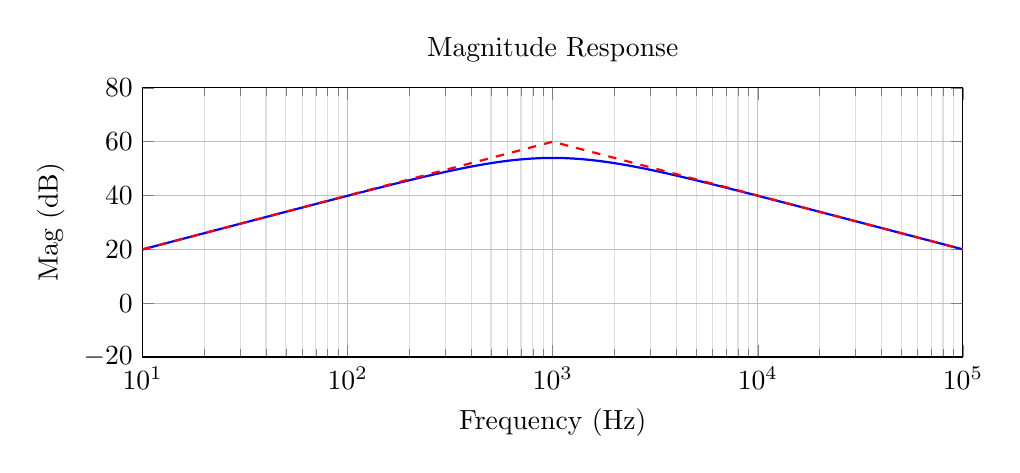
\begin{tikzpicture}
    \begin{semilogxaxis}[
        width=12cm, height=5cm,
        xmin=10, xmax=100000, ymin=-20, ymax=80,
        grid=both, minor grid style={gray!25}, major grid style={gray!50},
        ylabel={Mag (dB)}, xlabel={Frequency (Hz)},
        title={Magnitude Response}
    ]
    % EXACT (Blue Smooth)
    \addplot[blue, thick, domain=10:100000, samples=100] 
        {20*log10( (10*x/10) / ( 1+(x/1000)^2 ) )};

    % ASYMPTOTIC (Red Linear)
    \addplot[red, thick, dashed] coordinates {
        (10, 20) (1000, 60) (100000, 20)
    };
    \end{semilogxaxis}
    \end{tikzpicture}

    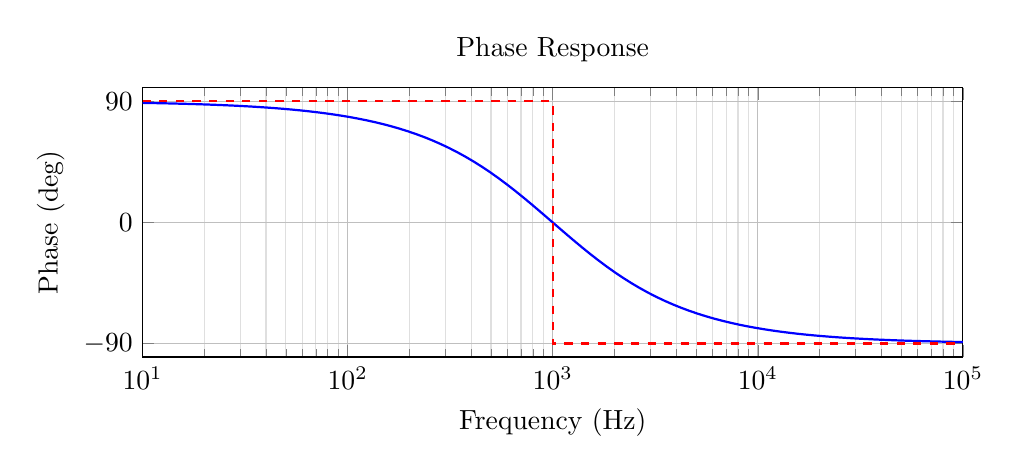
\begin{tikzpicture}
    \begin{semilogxaxis}[
        width=12cm, height=5cm,
        xmin=10, xmax=100000, ymin=-100, ymax=100,
        grid=both, minor grid style={gray!25}, major grid style={gray!50},
        ylabel={Phase (deg)}, xlabel={Frequency (Hz)},
        ytick={90, 0, -90},
        title={Phase Response}
    ]
    % EXACT (Blue Smooth)
    \addplot[blue, thick, domain=10:100000, samples=100] 
        {90 - 2*atan(x/1000)};

    % ASYMPTOTIC (Red Linear)
    \addplot[red, thick, dashed] coordinates {
        (10, 90) (1000, 90) (1000, -90) (100000, -90)
    };
    \end{semilogxaxis}
    \end{tikzpicture}

    \textbf{Step-by-Step Derivation:}
    \begin{enumerate}
        \item \textbf{Identify Poles/Zeros:}
        \begin{itemize}
            \item Numerator: Single zero at origin. Slope $+20$ dB/dec.
            \item Denominator: \textbf{Double Pole} at $1$ kHz.
        \end{itemize}
        
        \item \textbf{Calculate Reference Gain:}
        Evaluate at a frequency before the pole, e.g., $f=10$ Hz.
        \[ |H(10)| \approx \frac{10 \cdot (10/10)}{1} = 10 \implies 20\log(10) = \textbf{20 dB}. \]
        
        \item \textbf{Construct Magnitude Plot:}
        \begin{itemize}
            \item \textbf{Start (10 Hz):} 20 dB. Slope is $+20$ dB/dec (due to zero).
            \item \textbf{At 1 kHz:} We traveled 2 decades ($10 \to 1k$). Gain rises $20 \times 2 = 40$dB. Peak gain is $20+40=60$dB.
            \item \textbf{Corner 1 (1 kHz):} Double pole kicks in. Slope change is $2 \times -20 = -40$.
            \item \textbf{New Slope:} Current slope was $+20$. Change is $-40$. Final slope: $20 - 40 = \textbf{-20 dB/dec}$.
        \end{itemize}

        \item \textbf{Construct Phase Plot:}
        \begin{itemize}
            \item \textbf{Start:} Single zero at origin gives constant $+90^\circ$.
            \item \textbf{Transition:} Double pole at 1 kHz causes a drop of $2 \times 90 = 180^\circ$.
            \item \textbf{End:} $+90^\circ - 180^\circ = -90^\circ$.
        \end{itemize}
    \end{enumerate}
\end{answer}

    \qnewpage

    % --- PROBLEM 1b ---
\end{partquestion}

% =========================================================
\begin{partquestion}{secondsystem}
{Consider the system:
    \[ H(f) = \frac{10 \cdot (j\frac{f}{10\text{Hz}})^2}{(1 + j\frac{f}{100\text{Hz}})(1 + j\frac{f}{10\text{kHz}})} \]
    
    \textbf{Analysis, Derivation, and Sketch:}}

\begin{answer}
    \textbf{Visual Solution:}
    
    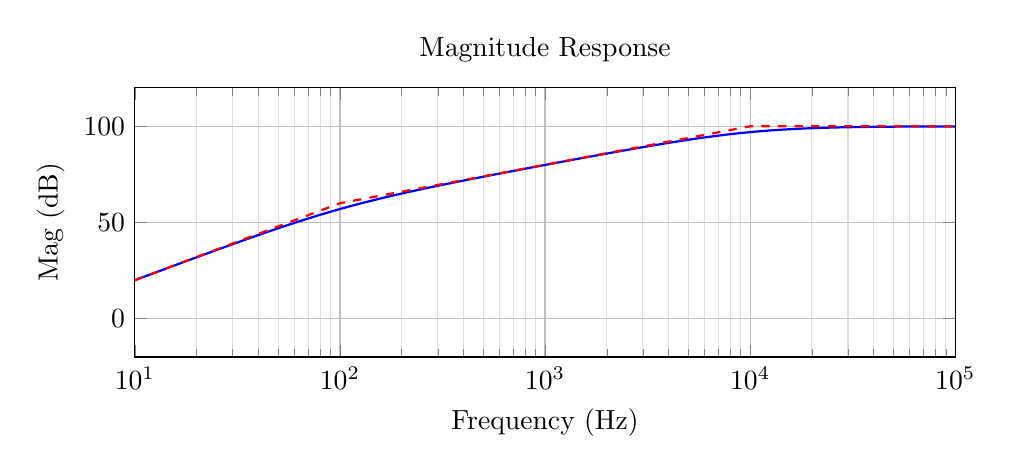
\begin{tikzpicture}
    \begin{semilogxaxis}[
        width=12cm, height=5cm,
        xmin=10, xmax=100000, ymin=-20, ymax=120,
        grid=both, minor grid style={gray!25}, major grid style={gray!50},
        ylabel={Mag (dB)}, xlabel={Frequency (Hz)},
        title={Magnitude Response}
    ]
    % EXACT (Blue Smooth)
    \addplot[blue, thick, domain=10:100000, samples=100] 
        {20*log10( (10*(x/10)^2) / (sqrt(1+(x/100)^2) * sqrt(1+(x/10000)^2)) )};
    
    % ASYMPTOTIC (Red Linear)
    \addplot[red, thick, dashed] coordinates {
        (10, 20) (100, 60) (10000, 100) (100000, 100)
    };
    \end{semilogxaxis}
    \end{tikzpicture}
    
    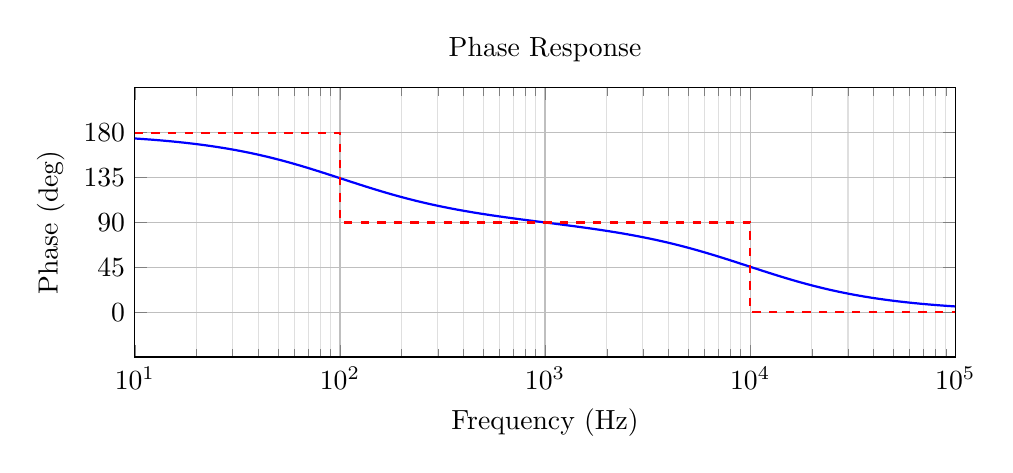
\begin{tikzpicture}
    \begin{semilogxaxis}[
        width=12cm, height=5cm,
        xmin=10, xmax=100000, ymin=-45, ymax=225,
        grid=both, minor grid style={gray!25}, major grid style={gray!50},
        ylabel={Phase (deg)}, xlabel={Frequency (Hz)},
        ytick={0, 45, 90, 135, 180},
        title={Phase Response}
    ]
    % EXACT (Blue Smooth)
    \addplot[blue, thick, domain=10:100000, samples=100] 
        {180 - atan(x/100) - atan(x/10000)};

    % ASYMPTOTIC (Red Linear)
    \addplot[red, thick, dashed] coordinates {
        (10, 180) (100, 180) (100, 90) (10000, 90) (10000, 0) (100000, 0)
    };
    \end{semilogxaxis}
    \end{tikzpicture}

    \textbf{Step-by-Step Derivation:}
    \begin{enumerate}
        \item \textbf{Identify Poles/Zeros:}
        \begin{itemize}
            \item Numerator: $(j\frac{f}{10})^2$ indicates a \textbf{double zero at the origin}. This sets the starting slope to $+40$ dB/dec.
            \item Denominator: Poles at $f_{p1} = 100\text{Hz}$ and $f_{p2} = 10\text{kHz}$.
        \end{itemize}
        
        \item \textbf{Calculate Reference Gain:}
        Since there is a zero at the origin, DC gain is $-\infty$ dB. We calculate gain at a specific frequency, e.g., $f=10\text{Hz}$.
        \[ |H(10)| \approx \frac{10 \cdot (10/10)^2}{1 \cdot 1} = 10 \implies 20\log(10) = \textbf{20 dB at 10Hz}. \]
        
        \item \textbf{Construct Magnitude Plot:}
        \begin{itemize}
            \item \textbf{Start:} At 10Hz, gain is 20dB. Slope is $+40$ dB/dec (double zero).
            \item \textbf{At 100 Hz:} We have moved 1 decade. Gain rises by 40dB ($20+40=60$dB). We hit the first pole ($100$Hz), which reduces the slope by 20. New slope: $+20$ dB/dec.
            \item \textbf{At 10 kHz:} We have moved 2 decades ($100 \to 10k$). Gain rises by $20 \times 2 = 40$dB ($60+40=100$dB). We hit the second pole ($10k$Hz), which reduces slope by another 20. New slope: $0$ dB/dec (Flat).
        \end{itemize}

        \item \textbf{Construct Phase Plot:}
        \begin{itemize}
            \item \textbf{Start:} A double zero ($j^2$) gives a constant phase of $+180^\circ$.
            \item \textbf{Transitions:} At $f_{p1}=100$Hz, phase drops by $90^\circ$ (to $+90^\circ$). At $f_{p2}=10$kHz, phase drops another $90^\circ$ (to $0^\circ$).
        \end{itemize}
    \end{enumerate}
\end{answer}

    \qnewpage

    % --- PROBLEM 1c ---
\end{partquestion}

% =========================================================
\begin{partquestion}{thirdsystem}
{Consider the system:
    \[ H(f) = \frac{100}{(1 + j\frac{f}{100\text{Hz}})(1 + j\frac{f}{2\text{kHz}})^2} \]
    
    \textbf{Analysis, Derivation, and Sketch:}}

\begin{answer}
    \textbf{Visual Solution:}

    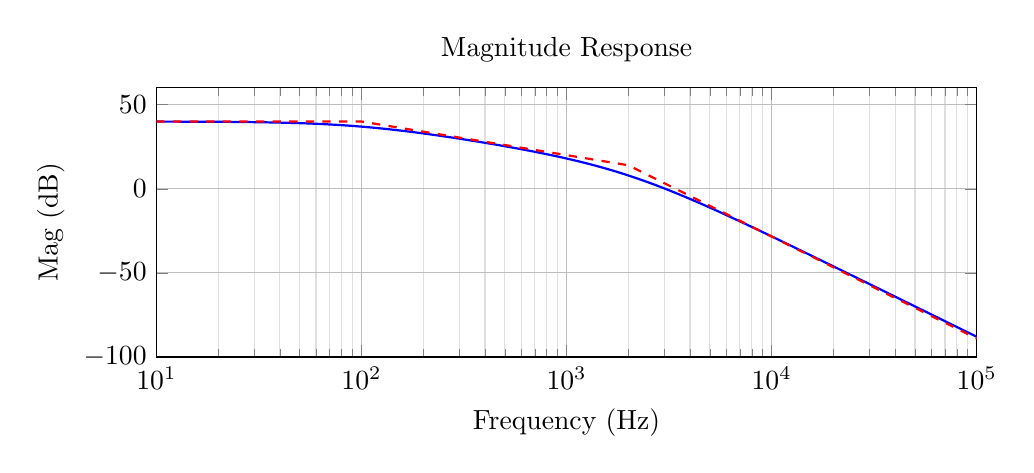
\begin{tikzpicture}
    \begin{semilogxaxis}[
        width=12cm, height=5cm,
        xmin=10, xmax=100000, ymin=-100, ymax=60,
        grid=both, minor grid style={gray!25}, major grid style={gray!50},
        ylabel={Mag (dB)}, xlabel={Frequency (Hz)},
        title={Magnitude Response}
    ]
    % EXACT (Blue Smooth)
    \addplot[blue, thick, domain=10:100000, samples=100] 
        {20*log10( 100 / (sqrt(1+(x/100)^2) * (1+(x/2000)^2)) )};

    % ASYMPTOTIC (Red Linear)
    \addplot[red, thick, dashed] coordinates {
        (10, 40) (100, 40) (2000, 14) (100000, -89)
    };
    \end{semilogxaxis}
    \end{tikzpicture}

    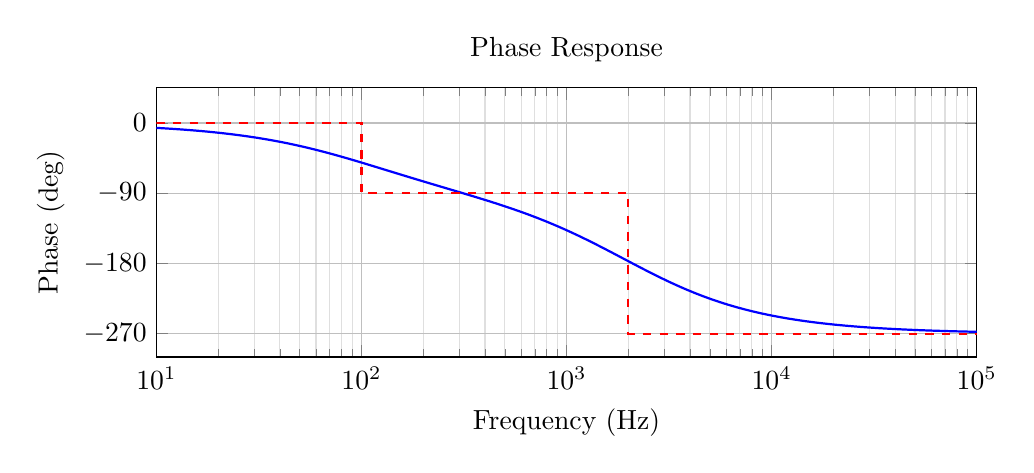
\begin{tikzpicture}
    \begin{semilogxaxis}[
        width=12cm, height=5cm,
        xmin=10, xmax=100000, ymin=-300, ymax=45,
        grid=both, minor grid style={gray!25}, major grid style={gray!50},
        ylabel={Phase (deg)}, xlabel={Frequency (Hz)},
        ytick={0, -90, -180, -270},
        title={Phase Response}
    ]
    % EXACT (Blue Smooth)
    \addplot[blue, thick, domain=10:100000, samples=100] 
        {0 - atan(x/100) - 2*atan(x/2000)};

    % ASYMPTOTIC (Red Linear)
    \addplot[red, thick, dashed] coordinates {
        (10, 0) (100, 0) (100, -90) (2000, -90) (2000, -270) (100000, -270)
    };
    \end{semilogxaxis}
    \end{tikzpicture}

    \textbf{Step-by-Step Derivation:}
    \begin{enumerate}
        \item \textbf{Calculate DC Gain:}
        At low frequencies ($f \to 0$), the $j$ terms become 0.
        \[ H(0) = \frac{100}{(1)(1)^2} = 100 \implies 20\log(100) = \textbf{40 dB}. \]
        
        \item \textbf{Identify Poles/Zeros:}
        \begin{itemize}
            \item Single Pole at $100$ Hz.
            \item \textbf{Double Pole} at $2$ kHz.
        \end{itemize}

        \item \textbf{Construct Magnitude Plot:}
        \begin{itemize}
            \item \textbf{Region 1 ($<100$ Hz):} Flat at 40 dB.
            \item \textbf{Corner 1 ($100$ Hz):} Single pole starts. Slope changes $0 \to -20$ dB/dec.
            \item \textbf{Value at 2kHz:} From 100Hz to 2kHz is roughly 1.3 decades ($\log_{10}(20)$). The drop is $-20 \times 1.3 = -26$dB. Gain at 2kHz $\approx 40 - 26 = 14$ dB.
            \item \textbf{Corner 2 ($2$ kHz):} Double pole kicks in. This adds $-40$ dB/dec to the slope. New slope: $-20 + (-40) = \textbf{-60 dB/dec}$.
        \end{itemize}
        
        \item \textbf{Construct Phase Plot:}
        \begin{itemize}
            \item Starts at $0^\circ$.
            \item At 100 Hz: Phase drops $0^\circ \to -90^\circ$.
            \item At 2 kHz: Double pole causes a double drop ($2 \times -90^\circ$). Phase goes from $-90^\circ \to -270^\circ$.
        \end{itemize}
    \end{enumerate}
\end{answer}

\end{partquestion}

\end{mainquestion}
